\subsection{Astrobiology System Design}
\label{sec:Astrobiology Design}

The collection assembly will be designed as a multi-compartment structure, with various collection and control containers, two pumps, two pump heaters, and two solenoids.  The control containers will be connected to a solenoid that will remain closed until post-sanitation procedures are performed. The sample collection containers will be connected to a vacuum pump located outside of the clean box structure.  One of the chambers will be a non-liquid collection container. Heaters will be attached to the pumps to aid during a cold start. Once float altitude is reached, the solenoids connected to the sample collection containers will be opened and the pumps will be powered on; allowing air to flow to the collection containers.The containers will hold a range of amounts and concentrations, \SIrange{30}{60}{\milli\liter} of \SIrange{15}{30}{\%} sterile glycerol solutions. A 316 Stainless Steel \SI{1/4}{\inch} NPT Vent to Atmosphere Vitron Seal Valve will be embedded in each of the compartments, to accommodate for the pressure changes that occurs with the variations in altitude over the course of a flight~\cite{valve}, as well as operate as the sample exhaust.  The left side of Figure~\ref{fig:pump} displays the collection assembly with the openings for the sample and exhaust tubing, while the right side of Figure~\ref{fig:pump} shows the 3D rendering of the sampling pump.  

\begin{figure}[!h] 
\begin{center}
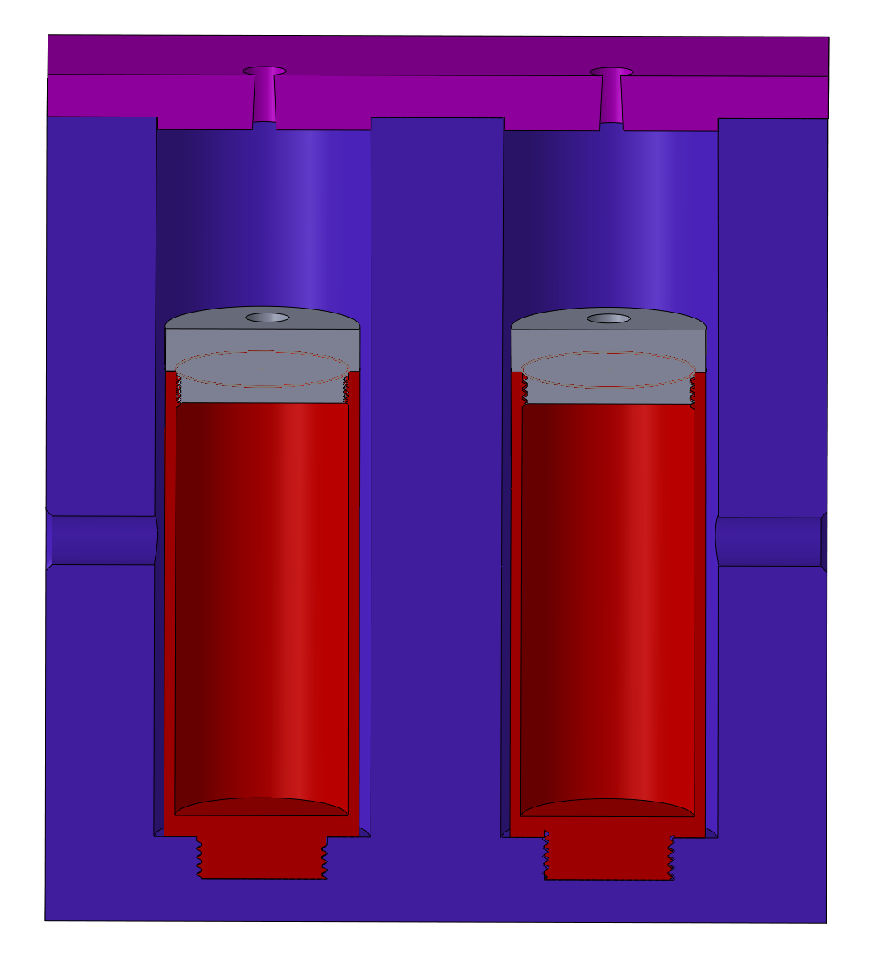
\includegraphics[scale=.4]{./Figures/CB.PDF}
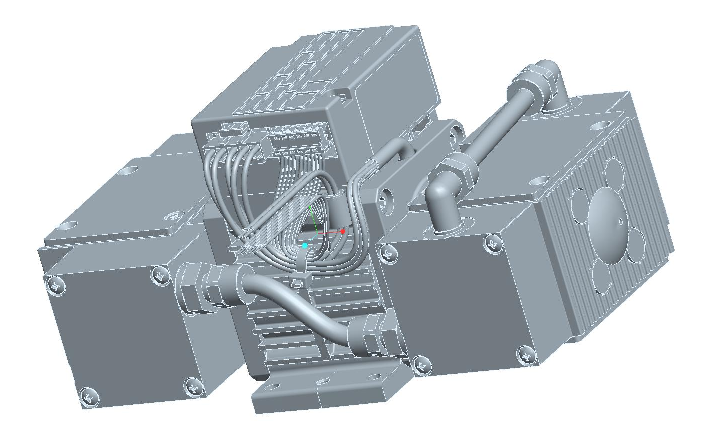
\includegraphics[scale=.8]{./Figures/Pump.pdf}
\caption{{\bf Left:} Cross-section view of the clean box with experimental and control containers. {\bf Right:} KNF N84-4 commercial gas-sampling diaphragm vacuum pump.}
\label{fig:pump}
\end{center}
\end{figure} 
